\documentclass[12pt]{article}
\usepackage[english]{babel}
\usepackage[utf8]{inputenc}

\usepackage{geometry}
\geometry{
	letterpaper, 
	portrait, 
	top=.75in,
	left=.8in,
	right=.75in,
	bottom=.5in		} 	% Page Margins
	
%% additional packages for nice things
\usepackage{amsmath} 	% for most math
\usepackage{commath} 	% for abs
\usepackage{lastpage}	% for page count
\usepackage{amssymb} 	% for therefore
\usepackage{graphicx} 	% for image handling
\usepackage{wrapfig} 	% wrap figures
\usepackage[none]{hyphenat} % for no hyphenations
\usepackage{booktabs} 	% enhanced table qualities
\usepackage{array} 		% for >{} column characterisctis
\usepackage{physics} 	% for easier derivative \dv....
\usepackage{tikz} 		% for graphic@!
\usepackage{circuitikz} % for circuits!
\usetikzlibrary{arrows.meta} % for loads
\usepackage[thicklines]{cancel}	% for cancels
\usepackage{xcolor}		% for color cancels
\usepackage[per-mode=fraction]{siunitx} % for si units and num
\usepackage{fancyhdr} 	% for header
\usepackage{comment}	% for ability to comment out large sections
\usepackage{multicol}	% for multiple columns using multicols
\usepackage[framed,numbered]{matlab-prettifier} % matlab sytle listing
\usepackage{marvosym} 	% for boltsymbol lightning
\usepackage{pdflscape} 	% for various landscape pages in portrait docs.
\usepackage{float}
\usepackage{fancyvrb}	% for Verbatim (a tab respecting verbatim)
\usepackage{enumitem}	% for [resume] functionality of enumerate
\usepackage{subfigure}

%% package config 
\sisetup{output-exponent-marker=\ensuremath{\mathrm{E}}} % for engineer E
\renewcommand{\CancelColor}{\color{red}}	% for color cancels
\lstset{aboveskip=2pt,belowskip=2pt} % for more compact table
\def\arraystretch{1.4} % adjust size of arrays
%\arraycolsep=1.4pt\def
\setlength{\parindent}{0cm} % Remove indentation from paragraphs
\setlength{\columnsep}{0.5cm}
\lstset{
	style      = Matlab-editor,
	basicstyle = \ttfamily\footnotesize, % if you want to use Courier - not really used?
}
\renewcommand*{\pd}[3][]{\ensuremath{\dfrac{\partial^{#1} #2}{\partial #3}}} % for larger pd fracs
\renewcommand{\real}[1]{\mathbb{R}\left\{ #1 \right\}}	% for REAL symbol
\newcommand{\imag}[1]{\mathbb{I}\left\{ #1 \right\}}	% for IMAG symbol
\definecolor{m}{rgb}{1,0,1}	% for MATLAB matching magenta
	
%% custom macros
\newcommand\numberthis{\addtocounter{equation}{1}\tag{\theequation}} % for simple \numberthis command
\newcommand{\equal}{=} % so circuitikz can have an = in the labels
\newcolumntype{L}[1]{>{\raggedright\let\newline\\\arraybackslash\hspace{0pt}}m{#1}}
\newcolumntype{C}[1]{>{\centering\let\newline\\\arraybackslash\hspace{0pt}}m{#1}}
\newcolumntype{R}[1]{>{\raggedleft\let\newline\\\arraybackslash\hspace{0pt}}m{#1}}

%% Header
\pagestyle{fancy} % for header stuffs
\fancyhf{}
\rhead{Thad Haines \\ Page \thepage\ of \pageref{LastPage}}
\chead{ggov1 Model Progress \\ Matt Approach}
\lhead{Research \\ }
% spacing
\headheight 29 pt
\headsep 6 pt

\newcommand{\figW}{1}
\newcommand{\figH}{.26}
\documentclass[]{standalone}
\usepackage{tikz}
\usetikzlibrary{shapes,arrows,calc,positioning}
\usepackage{amsmath} % for dfrac

% definition of basic block
\tikzset{
    block/.style = {draw, rectangle,
        minimum height=1.2cm,
        minimum width=2cm},
    input/.style = {coordinate,node distance=1cm},
    output/.style = {coordinate,node distance=1cm},
    sum/.style = {draw, circle, node distance=1cm},
}

% definition of saturation block
\tikzset{% from https://tex.stackexchange.com/questions/161075/saturation-block
  saturation block/.style={%
    draw, 
    path picture={
      % Get the width and height of the path picture node
      \pgfpointdiff{\pgfpointanchor{path picture bounding box}{north east}}%
        {\pgfpointanchor{path picture bounding box}{south west}}
      \pgfgetlastxy\x\y
      % Scale the x and y vectors so that the range
      % -1 to 1 is slightly shorter than the size of the node
      \tikzset{x=\x*.4, y=\y*.4}
      %
      % Draw annotation
      \draw (-1,0) -- (1,0) (0,-1) -- (0,1); 
      \draw (-1,-.7) -- (-.6,-.7) -- (.6,.7) -- (1,.7);
    }
  }
}

\begin{document}
	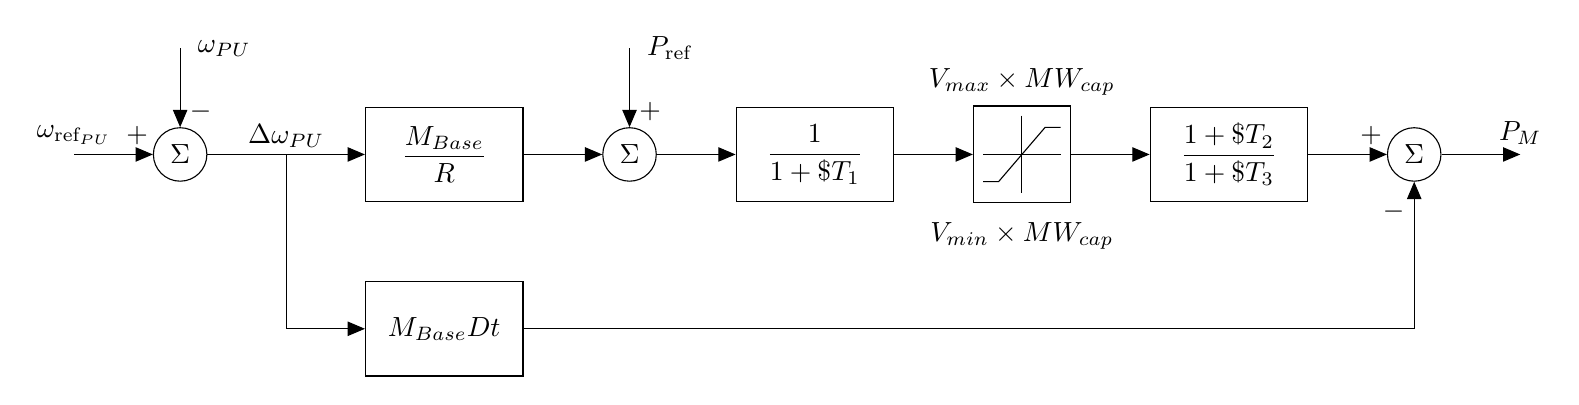
\begin{tikzpicture}[auto, node distance=1cm,>=triangle 45]
		% Starting input (wref)
		\node [input, name=input, label=$\omega_{\text{ref}_{PU}}$] {};
		% sum 1
		\node [sum, right=of input] (sum1) {$\Sigma$};
		% delta w node and label
		\coordinate [right=of sum1]  (deltaw) {};
		\node [above=-.8em of deltaw,label={$\Delta\omega_{PU}$}]  (deltaWlabel){};
		% delta w gain blocks
		\node [block, right=of deltaw] (gain) {$\dfrac{M_{Base}}{R}$};
		\node [block, below=of gain] (Dt) {$M_{Base} Dt$};
		% Pref sum
		\node [sum, right=of gain] (sumP) {$\Sigma$};
		% Valve state block
		\node [block, right=of sumP] (state1) {$\dfrac{1}{1+\$T_1}$};
		% limiter and labels
		\node [saturation block, right=of state1 , minimum size=3.5em, label=$V_{max} \times MW_{cap}$] (mwcap){};
		\node [below=2em of mwcap, label=$V_{min} \times MW_{cap}$](mwcapLOW){};
		% turbine state
		\node [block, right=of mwcap] (state2) {$\dfrac{1+\$T_2}{1+\$T_3}$};
		% damping sum
		\node [sum, right= of state2] (sum2) {$\Sigma$};
		% Pm out
		\node [output, right=of sum2, label=$P_M$] (output) {};
		% w and pref in
		\node [input, name=omega, above= of sum1,label={[label distance=.1cm]0:$\omega_{PU}$} ] {};
		\node [input, name=Pref, above= of sumP,label={[label distance=.1cm]0:$P_{\text{ref}}$} ] {};

		% connecting lines
		\draw [draw,->] (input) -- node[pos=0.8] {$+$} (sum1); % straight connecting line
		\draw [->] (omega) -- node[pos=0.8] {$-$} (sum1);
		\draw [->] (Pref) -- node[pos=0.8] {$+$} (sumP);
		\draw [->] (sum1) -- (gain) ;
		\draw [->] (gain) -- (sumP) ;
		\draw [->] (sumP) -- (state1) ;
		\draw [->] (state1) -- (mwcap) ;
		\draw [->] (mwcap) -- (state2) ;
		\draw [->] (state2) -- node[pos=0.8] {$+$} (sum2);
		\draw [->] (deltaw) |-  (Dt); % line goes down and across
		\draw [->] (Dt) -|  node[pos=0.9] {$-$} (sum2); % line goes across then down
		\draw [->] (sum2) -- (output);
	\end{tikzpicture} 
\end{document}
\begin{document}
\paragraph{Matt Approach:} Pick time constants from ggov1 model to put into the tgov1 model.

	\begin{figure}[h!]
			\centering
			\includegraphics[width=\linewidth]{tgov1}\vspace{-1em}
			\caption{LTD tgov1 Model.}
			\label{tgov1}		 
	\end{figure}\vspace{-1em}

	\begin{figure}[h!]
				\centering
				\includegraphics[width=\linewidth]{psds_ggox1}  \vspace{-2em}
				\caption{PSDS ggov1 Model} 
				\label{ggov1}
	\end{figure}\vspace{-2em}

\paragraph{Results:} While this was relatively easy to do, and the required parsing of ggov1 infromation from the .dyd is useful - dynamic testing shows that this is not a very accurate dynamic approach. Steady state results match in all cases tested. Probably need to use an alternative approach.

\begin{table}[!h]
	\begin{tabular}{l l l l}
	T1 & T2 & T3 & Result \\ \toprule
Ta & Tc & Tb & Faster response than desired, minimal overshoot.(Figure~\ref{TaTcTb})\\
Tact & Tc & Tb & Similar to Ta Tc Tb case, slightly more overshoot \\
Tpelec & Tc & Tb & Faster and more overshoot than desired. (Figure~\ref{TpelecTcTb})\\
Tpelec & Tc & Tact & Similar to Tpeclec Tc Tb case, less damping (more overshoot) 
	\end{tabular}
\end{table}
\pagebreak

	\begin{figure}[h!]	
				\centering
				\includegraphics[width=\figW\linewidth]{TaTcTb}  \vspace{-1.5em}
				\caption{PSDS and LTD results. Case: T1=Ta, T2=Tc, T3=Tb}
				\label{TaTcTb}
	\end{figure}

	\begin{figure}[h!]	
				\centering
				\includegraphics[width=\figW\linewidth]{TpelecTcTb}  \vspace{-1.5em}
				\caption{PSDS and LTD results. Case: T1=Tpelec, T2=Tc, T3=Tb}
				\label{TpelecTcTb}
	\end{figure}



\end{document}
